\section{Concept}

Lorem ipsum dolor sit amet, consectetur adipiscing elit. Nullam hendrerit interdum sagittis. Nulla facilisi. Pellentesque laoreet tincidunt semper. Pellentesque pellentesque lectus id arcu interdum cursus ut ac dui. Etiam feugiat nisl ac odio suscipit pretium venenatis eget diam. Morbi molestie ipsum sit amet sapien rutrum luctus. Proin ac dolor ut metus laoreet aliquam non id nunc. Curabitur non efficitur dolor. Donec iaculis, dui et porta iaculis, magna tellus placerat ex, sed porta sem ligula ac augue. Fusce vitae sagittis ex. Pellentesque faucibus cursus elit, et faucibus velit cursus in. Nam lobortis id neque id hendrerit. Fusce et dolor nisi.


\subsection{Use case diagram}

\begin{figure}[h]
	\centering
	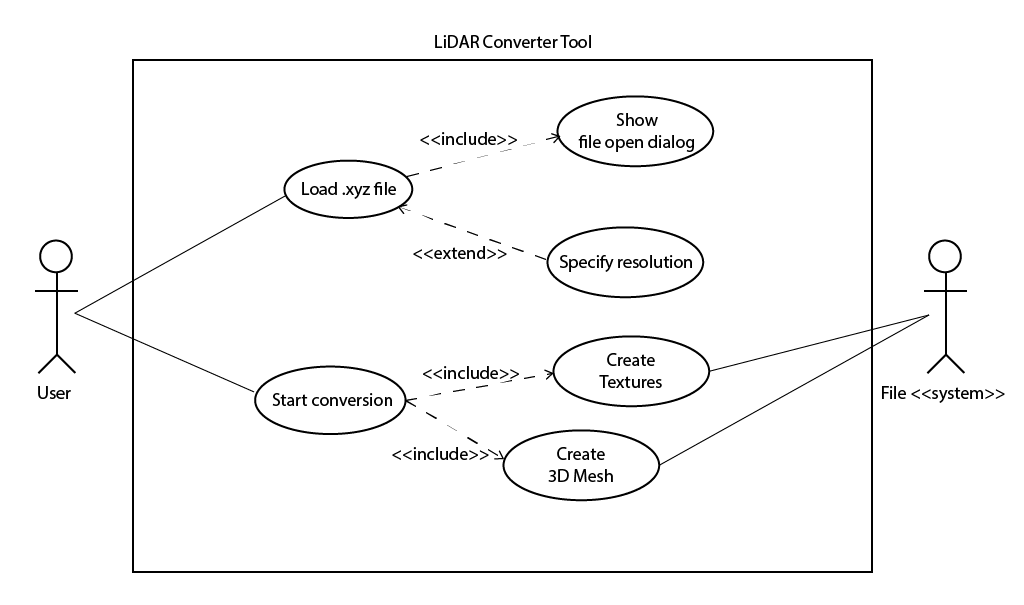
\includegraphics[scale=0.4]{UseCaseDiagram_PC2B.png}
	\caption{Use Case Diagram}
	\label{fig:use_case}
\end{figure}


\subsection{Laser scanning on location}

Cum sociis natoque penatibus et magnis dis parturient montes, nascetur ridiculus mus. Donec non auctor sem, sit amet fringilla purus. Phasellus eu orci et nibh lobortis faucibus id vel lorem. Aliquam ut diam id mi aliquam finibus eu id neque. Nam consequat efficitur mi sed maximus. Nullam egestas neque enim. Nulla nec eleifend mauris, eget sollicitudin velit. Quisque ultricies feugiat neque ut condimentum. Aliquam vehicula faucibus sapien non convallis. Nullam consectetur sagittis sollicitudin. Nulla mollis laoreet metus et consectetur.

\begin{figure}[h]
	\centering
	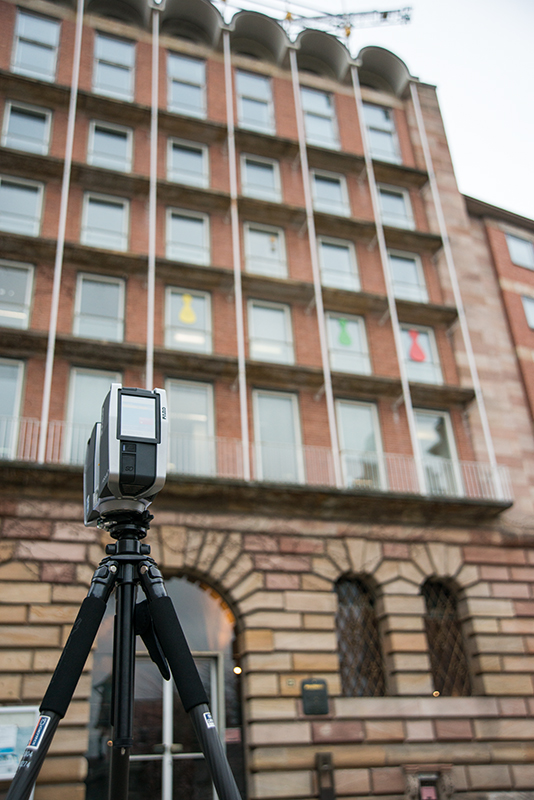
\includegraphics[scale=0.4]{PellerhausLaserScan.jpg}
	\caption{Scanning with Faro Focus 3D}
	\label{fig:laser_scanning_on_location}
\end{figure}



\begin{table}[h]
	\centering
	\begin{tabular}{l | l | l}
		A & B & C \\
		\hline
		1 & 3 & 4 \\
		1 & 3 & 4 \\
	\end{tabular}
	\caption{very basic table caption}
	\label{tab:abc}
\end{table}



\section{Generating data and testing algorithms}

\subsection{BlenSor}

Etiam non volutpat diam. Nam ac consectetur felis. Ut nec mi dictum, lobortis mauris quis, dapibus ligula. Nulla porttitor diam sed mauris dapibus posuere. Fusce pellentesque odio at nisl placerat porta. Donec urna risus, iaculis vitae justo quis, tempus ullamcorper diam. Integer eu gravida est. Phasellus eu ex tincidunt urna tempus pulvinar in in metus. Mauris tempus magna ac finibus suscipit. Praesent malesuada magna nibh, at rutrum felis semper a.

\subsection{Test-Addon for Blender}

Etiam non volutpat diam. Nam ac consectetur felis. Ut nec mi dictum, lobortis mauris quis, dapibus ligula. Nulla porttitor diam sed mauris dapibus posuere. Fusce pellentesque odio at nisl placerat porta. Donec urna risus, iaculis vitae justo quis, tempus ullamcorper diam. Integer eu gravida est. Phasellus eu ex tincidunt urna tempus pulvinar in in metus. Mauris tempus magna ac finibus suscipit. Praesent malesuada magna nibh, at rutrum felis semper a.

\section{Prototype}

\subsection{Point Cloud Importer}

Etiam non volutpat diam. Nam ac consectetur felis. Ut nec mi dictum, lobortis mauris quis, dapibus ligula. Nulla porttitor diam sed mauris dapibus posuere. Fusce pellentesque odio at nisl placerat porta. Donec urna risus, iaculis vitae justo quis, tempus ullamcorper diam. Integer eu gravida est. Phasellus eu ex tincidunt urna tempus pulvinar in in metus. Mauris tempus magna ac finibus suscipit. Praesent malesuada magna nibh, at rutrum felis semper a.

\subsubsection{Point Cloud data formats}

\begin{table}[h]
	\centering
	\begin{subtable}[h]{0.45\textwidth}
		\centering
		\begin{tabular}{l | l | l}
			Day & Max Temp & Min temp \\
			\hline \hline
			Mon & 20 & 13 \\
			Tue & 22 & 14 \\
			Wed & 23 & 12 \\
			Thu & 25 & 13 \\
			Fri & 18 & 7 \\
			Sat & 15 & 13 \\
			Sun & 20 & 13
		\end{tabular}
		\caption{First Week}
		\label{tab:week1}
	\end{subtable}
	\hfill
	\begin{subtable}[h]{0.45\textwidth}
		\centering
		\begin{tabular}{l | l | l}
			Day & Max Temp & Min Temp \\
			\hline \hline
			Mon & 17 & 11 \\
			Tue & 16 & 10 \\
			Wed & 14 & 8 \\
			Thu & 12 & 5 \\
			Fri & 15 & 7 \\
			Sat & 16 & 12 \\
			Sun & 15 & 9
		\end{tabular}
		\caption{Second Week}
		\label{tab:week2}
	\end{subtable}
	\caption{Max and min temp recorded during the first two weeks in January}
	\label{tab:temps}
\end{table}


\subsection{Projecting 3D points onto a 2D plane}


\subsection{Saving textures}


\subsection{OpenGL Point Cloud Viewer}

This russian video tutorial was very helpful with the basic setup with the Qt framework.

\cite{ytQtOpenGL}

\subsection{Performance Optimization}


\subsection{Meshing}

Interdum et malesuada fames ac ante ipsum primis in faucibus. Cras quis pharetra libero. Pellentesque consectetur, quam vel ultrices finibus, sem enim consectetur mi, in dictum tellus leo eu ante. Maecenas consequat egestas erat, in vestibulum velit pulvinar ac. Suspendisse ullamcorper augue sapien, ac suscipit nulla dictum in. Nam sit amet congue ipsum. Aenean non felis malesuada, feugiat lectus a, tincidunt quam. Fusce nec quam egestas, vulputate est in, commodo nisi. Phasellus id nunc sit amet quam iaculis ornare eu id libero. Ut tempor nisi sed est pretium auctor. Donec in nunc turpis. Integer non tristique dolor. Curabitur a elit mollis urna finibus scelerisque sit amet vel erat. Nullam nec maximus erat. Duis ante mi, posuere ut lobortis nec, posuere eu ligula.



\subsection{Mesh Exporter}

There are different formats, one had to be chosen that supported at least vertices and faces.

\subsubsection{.obj}

The .obj format is the most popular and can be one of the easiest to understand file formats to save 3D geometry with not only points, but vertices, normals, texture coordinates and much more. It was the first choice when testing mesh exporting from the converter software and examining it in Blender.

\subsubsection{.blend}

A personal goal for this research was to implement a .blend export feature to allow for a native importing of the panorama mesh into Blender. However, this goal was not reached in this project. As it turned out, exporting the binary Blender file format was quite complicated, due to it's versatile structure. An experienced Blender Developer, Jeroen Bakker, stated in 2009 “When implementing loading and saving blend-files in a custom tool the difficulty is the opposite. In a custom tool loading a blend-file is easy, and saving a blend-file is difficult.” \parencite[see]{webMysteryOfTheBlend}. At least implementing it with the limited time for the thesis it was not feasable.



\subsubsection{custom format}

Even the Blender community suggested to not use the .blend format directly, but rather try a custom binary format. \parencite[compare]{webBlenderArtistsBlendExport}